\documentclass[11pt]{exam}
\usepackage[margin=1in]{geometry}
\pagestyle{plain}
\usepackage{amsmath,amsfonts,amssymb,amsthm,enumerate}
\usepackage{multicol}
\usepackage[]{graphicx}
\usepackage{hyperref}
\usepackage{tikz}
\usepackage{pgfplots}
\usepackage{subfigure}
\usepackage[final]{pdfpages}
\usetikzlibrary{angles,quotes}

\newcommand{\ddx}{\frac{d}{dx}}
\addtolength{\footskip}{2\baselineskip} % to lower the page numbers
\title{\vspace{-0.5in} Math 115 \\ Worksheet Section 3.6}
\date{}


% \theoremstyle{definition}
% \newtheorem{problem}{Problem}
\renewcommand{\questionlabel}{\textbf{Problem~\thequestion.}}
%\printanswers

\begin{document}
\maketitle
\vspace{-0.75in}
\begin{questions}
\question
  \begin{enumerate}[(a)]  
	\item Use the chain rule to differentiate (with respect to $x$) both sides of the identity $f\big(f^{-1}(x)\big) = x$.
	\item Having done that, solve for $\frac{d}{dx}f^{-1}(x)$.
	\item Now with this trick, find the derivatives (as functions of $x$) of the following functions.
\begin{multicols}{2}
\begin{enumerate}[(a)]
 \item $f(x)=\ln(x)$
 \item $f(x)=\log_{10} (x)$
 \item $f(x)=\arcsin(x)$
 \item $f(x)=\arctan(x)$
 \item $f(x) = \arccos(x)$
\end{enumerate}
\end{multicols}
\end{enumerate}
\begin{solution}
  We use the chain rule to find \[
    f'(f^{-1}(x))\cdot \ddx f^{-1}(x) = 1
  \]
  We then solve for \(\ddx f^{-1}(x)\) to get \[
    \ddx f^{-1}(x) = \frac{1}{f'(f^{-1}(x))}
  \]
  Finally, we check
  \begin{enumerate}[(a)]
  \item \(\ddx \ln(x) = \frac{1}{e^{\ln(x)}} = \frac{1}{x}\)
  \item \(\ddx \log_{10}(x) = \frac{1}{10^{\log_{10}(x)}\ln(10)} =
    \frac{1}{x \ln(10)}\)
  \item \(\ddx \arcsin(x) = \frac{1}{\cos(\arcsin(x))}\). Furthermore,
    using the following right triangle, we can solve \[
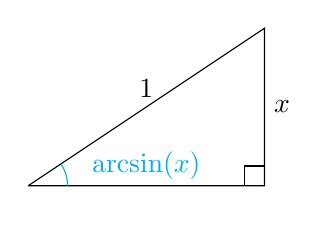
\begin{tikzpicture}[
  my angle/.style={
    every pic quotes/.append style={text=cyan},
    draw=cyan,
    angle radius=0.5cm,
  }]
  \coordinate (C) at (-1.5,-1);
  \coordinate (A) at (1.5,-1);
  \coordinate (B) at (1.5,1);
  \draw (C) -- node[above] {$1$} (B) -- node[right] {$x$} (A) -- node[below] {} (C);
  \draw (A) +(-.25,0) |- +(0,.25);
  \pic [my angle, ] {angle=A--C--B};
  \node at (0,-0.75) {\textcolor{cyan}{$\arcsin(x)$}};
\end{tikzpicture}
\implies \cos(\arcsin(x)) = \frac{\sqrt{1-x^2}}{1}
    \]
    Alternatively, we can use the identity that \(\cos(x) =
    \sqrt{1-\sin^2(x)}\) to get \(\cos(\arcsin(x)) = \sqrt{1-x^2}\).
    Thus, \(\arcsin(x) = \frac{1}{\sqrt{1-x^2}}\)
  \item \(\ddx \arctan(x) = \frac{1}{\sec^2(\arctan(x))}\), and we can
    solve \[
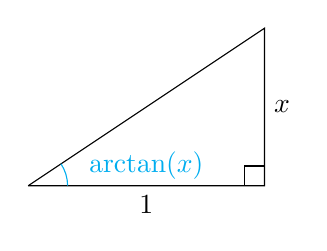
\begin{tikzpicture}[
  my angle/.style={
    every pic quotes/.append style={text=cyan},
    draw=cyan,
    angle radius=0.5cm,
  }]
  \coordinate (C) at (-1.5,-1);
  \coordinate (A) at (1.5,-1);
  \coordinate (B) at (1.5,1);
  \draw (C) -- node[above] {} (B) -- node[right] {$x$} (A) -- node[below] {\(1\)} (C);
  \draw (A) +(-.25,0) |- +(0,.25);
  \pic [my angle, ] {angle=A--C--B};
  \node at (0,-0.75) {\textcolor{cyan}{$\arctan(x)$}};
\end{tikzpicture}
\implies \sec^2(\arctan(x)) = (\sqrt{1^2+x^2})^2 = 1+x^2
    \]
    Alternatively, we can use the identity that \(\sec^2(x) =
    1+\tan^2(x)\) to get \(\sec^2(\arctan(x)) = 1+x^2\).
    Thus, \(\ddx \arctan = \frac{1}{1+x^2}\)
\item \(\ddx \arccos(x) = \frac{1}{-\sin(\arccos(x))}\), and we can
  solve \[
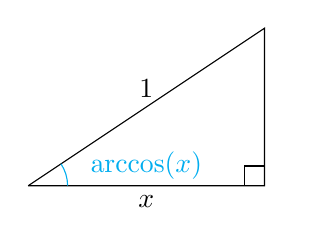
\begin{tikzpicture}[
  my angle/.style={
    every pic quotes/.append style={text=cyan},
    draw=cyan,
    angle radius=0.5cm,
  }]
  \coordinate (C) at (-1.5,-1);
  \coordinate (A) at (1.5,-1);
  \coordinate (B) at (1.5,1);
  \draw (C) -- node[above] {\(1\)} (B) -- node[right] {} (A) -- node[below] {\(x\)} (C);
  \draw (A) +(-.25,0) |- +(0,.25);
  \pic [my angle, ] {angle=A--C--B};
  \node at (0,-0.75) {\textcolor{cyan}{$\arccos(x)$}};
\end{tikzpicture}
\implies -\sin(\arccos(x)) = -\sqrt{1-x^2}
  \]
  and so \(\ddx \arccos(x) = -\frac{1}{\sqrt{1-x^2}}\)
  \end{enumerate}
\end{solution}
\question Consider the following graph of a function $f$ (solid line) and its inverse $f^{-1}$ (dotted line):

\vskip2ex

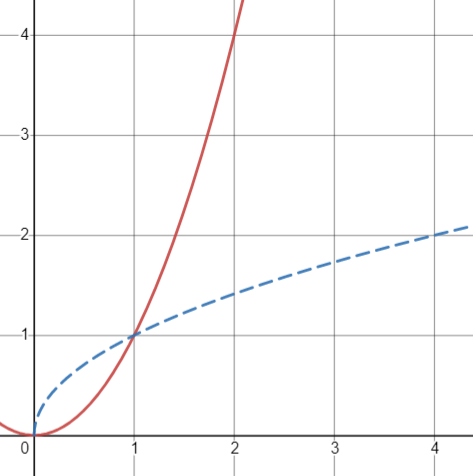
\includegraphics[width=2in]{Figures/ex.png}

\vskip2ex

Use the fact that $f'(2)=4$ and the general formula to find $\left(f^{-1}\right)'(4)$.  Then, use the graph to explain your answer. 
\begin{solution}
  Algebraically, we solve \[
    (f^{-1})'(4) = \frac{1}{f'(f^{-1}(4))} = \frac{1}{f'(2)} = \frac{1}{4}
  \]
  Geometrically, we see on the graph that, if we reflect \(y=f(x)\)
  over the line \(y=x\), then the tangent line for \(y = f(x)\) at
  \(x=2\) gets sent to the tangent line for \(x = f(2) = 4\) on
  \(y=f^{-1}(x)\) with the reciprocal slope \(\frac{1}{4}\).
\end{solution}
\question The number of years, \(T\), it takes an investment of
  \(\$1000\) to grow to \(\$F\) in an account which pays \(5\%\)
  interest compounded continuously is given by \[
    T = g(F) = 20\ln(0.001F)\,.
  \]
  Find \(g(5000)\) and \(g'(5000)\). Give units with your answers and
  interpret them in terms of money in the account.
  \begin{solution}
    \(g(5000) = 20 \ln(5) \approx 32.1\) years. This means it will
    take \(20\ln(5)\) years for \(\$1000\) to grow to \(\$5000\) with
    a \(5\%\) interest compounded continuously. 

    \(g'(F) =
    \frac{20}{0.001 F} \cdot 0.001 = \frac{20}{F}\). So, \(g'(5000) =
    \frac{20}{5000} = \frac{1}{250}\). This means that for the account
    to grow to \(\$5001\) instead of \(\$5000\), it will take
    approximately \(\frac{1}{250}\) more years (or about \(35\) hours).
  \end{solution}
\question At a particular location, \(f(p)\) is the number of gallons
  of gas sold when the price is \(p\) dollars per gallon.
  \begin{enumerate}[(a)]
  \item What does the statement \(f(2) = 4023\) tell you about gas sales?
  \item Find and interpret \(f^{-1}(4023)\).
  \item What does the statement \(f'(2) = -1250\) tell you about gas sales?
  \item Find and interpret \((f^{-1})'(4023)\).
  \end{enumerate}
  \begin{solution}
    \begin{enumerate}
    \item When gas costs \(\$2\) a gallon, \(4023\) gallons are sold.
    \item \(f^{-1}(4023) = 2\). When \(4023\) gallons of gas are sold, the
      price of gas was \(\$2\) a gallon.
    \item When the price of gas is increased from \(\$2\) to
      \(\$2.10\), approximately \(125\) fewer gallons of gas are sold.
    \item \((f^{-1})'(4023) = \frac{1}{f'(f^{-1}(4023))} =
      \frac{1}{f'(2)} = -\frac{1}{1250}\). This tells us when \(4024\)
      gallons of gas are sold instead of \(4023\) gallons, the price
      must be \(-\frac{1}{1250} = \$0.0008\) lower per gallon.
    \end{enumerate}
  \end{solution}
  \pagebreak
\question Solve the following textbook problems \\
  \vspace{-0.3in}
  \begin{multicols}{2}
\hspace*{-1cm}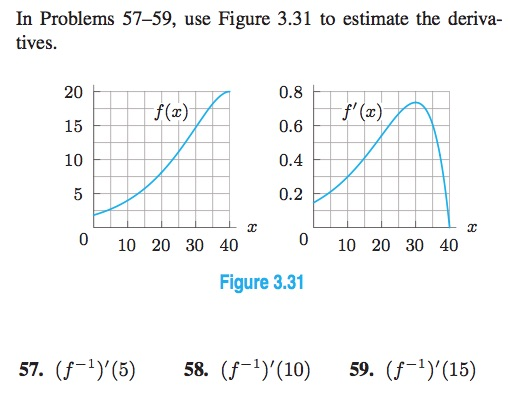
\includegraphics[width=3.7in]{Figures/no57to59.jpg}


\columnbreak

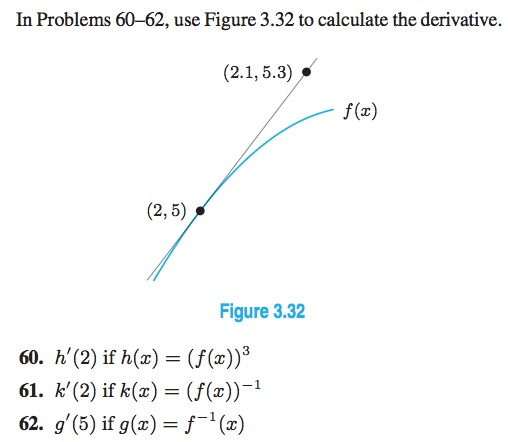
\includegraphics[width=3.7in]{Figures/no60to62.jpg}
\end{multicols}
\begin{solution}
  \begin{enumerate}
  \item[57.] \(f^{-1}(5) \approx 12 \implies (f^{-1})'(5) \approx \frac{1}{f'(12)} \approx \frac{1}{0.35} \approx 2.8\)
  \item[58.] \(f^{-1}(10) \approx 24 \implies (f^{-1})'(10) \approx \frac{1}{f'(24)} \approx \frac{1}{0.65} \approx 1.5\)
  \item[59.]\(f^{-1}(15) \approx 30 \implies (f^{-1})'(15) \approx \frac{1}{f'(30)} \approx \frac{1}{0.72} \approx 1.4\) 
  \item[60.] \(h'(x) = 3(f(x))^2 \cdot f'(x) \implies h'(2) = 3(5)^2
    \cdot 3\) since \(f'(2) = 3\).
  \item[61.] \(k'(x) = -(f(x))^{-2} \cdot f'(x) \implies -(f(2))^{-2}
    \cdot f'(2) = -(5)^{-2} \cdot 3 = -\frac{3}{25}\)
  \item[62.] \(g'(x) = \frac{1}{f'(f^{-1}(x))} \implies g'(5)=
    \frac{1}{f'(f^{-1}(5))} = \frac{1}{f'(2)} = \frac{1}{3}\)
  \end{enumerate}
\end{solution}
\question On what intervals is $\ln(x^2+1)$ concave up?
  \begin{solution}
    Let \(f(x) = \ln(x^2+1)\). We know \(f(x)\) is concave up if and
    only if \(f''(x) > 0\). Then, we compute
    \begin{align*}
      f'(x) & = \frac{2x}{x^2+1} \\
      f''(x) & = \frac{2(x^2+1)-2x(2x)}{(x^2+1)^2} \\
      & = \frac{2-2x^2}{(x^2+1)^2}
    \end{align*}
    Since \((x^2+1)^2 > 0\), we need only solve for \(2-2x^2 >
    0\). This is the same as \(1 > x^2\), so this happens
    only when \(-1 < x < 1\). Thus, \(f(x)\) is concave up on \((-1,1)\).
  \end{solution}
\question (Fall 2017 Exam 2) % problem 1
  Let \(A\) and \(B\) be two constants and
$$h(x) = \left\lbrace \begin{array}{ll} \!\! 2Bx + A \ln(x) & \textrm{if } 0 < x \leqslant 1 \\ \!\!\displaystyle\frac{4A}{x} + Bx - 1 & \textrm{if } 1 < x \leqslant 2 \end{array}\right.$$
Find all the values of $A$ and $B$ that make the function $h(x)$ differentiable on the interval $0 < x < 2$. If no such values exist, write none. Justify your answer.
\begin{solution}
  See \href{https://dhsp.math.lsa.umich.edu/exams/115exam2/f17/s9.pdf}{https://dhsp.math.lsa.umich.edu/exams/115exam2/f17/s9.pdf}
\end{solution}
\question (Winter 2018 Exam 2) %problem 1
  Some values of the twice differentiable function \(f(x)\) and of its first and second
derivative are given by the following table:
\begin{center}
  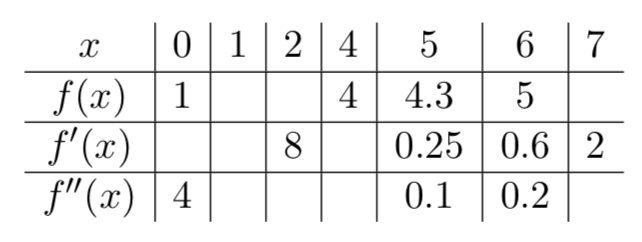
\includegraphics[scale=0.6]{Figures/table.png}
\end{center}
Suppose the function $f(x)$ is defined and invertible for $-\infty < x < \infty$. In the following questions, you will find some of the missing values using the information given. If there is not enough information given to answer the question, write “NEI”. Show your work.
\begin{enumerate}[(a)]
	\item The function $a(x) = \ln(1 + f(x))$ satisfies $a'(2) = 2$. Find $f(2)$.
	\item Let $b(x) = f(x) f'(x)$ and $b'(0)=4$. Find $f'(0)$.
	\item Let $h(x) = f^{-1}(x)$. Find the value of $h'(5)$.
\end{enumerate}
\begin{solution}
  See \href{https://dhsp.math.lsa.umich.edu/exams/115exam2/w18/s1.pdf}{https://dhsp.math.lsa.umich.edu/exams/115exam2/w18/s1.pdf}
\end{solution}
\question (Fall 2016 Exam 2) % problem 8
  Pepukai is studying the effect of the availability of water on the fruit productivity of Michigan apple trees. She observes that Michigan apple trees produce very few apples if they have too little water. She determines a function $p(w)$ that models the total weight, in pounds, of all the apples that an average Michigan apple tree produces in a season when it is watered with w gallons of water every week. The domain of p is $[5, 40]$. Some values of the function p and its derivative $p'$ are shown in the table below.
  \begin{center}
    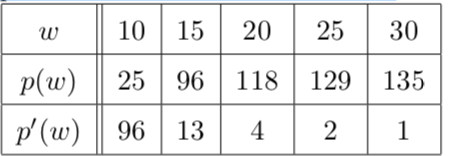
\includegraphics[scale=0.35]{Figures/table3.png}
  \end{center}
	The function \(p\) is invertible and the functions $p$, $p'$, and $p^{-1}$ are all differentiable. Furthermore, the function $p'$ is always decreasing.
	\begin{enumerate}[(a)]
	\item Find $(p^{-1})'(96)$.
	\item Circle the one statement that is best supported by the equation
	$$(p^{-1})'(10) = 0.01$$
	\begin{enumerate}[(i)]
	\item To increase the total weight of apples produced in a season by an average Michigan apple tree from 10 pounds to 11 pounds, the tree should be watered with about 0.01 additional gallons of water every week.
	\item If an average Michigan apple tree produces 10 pounds of apples in a season, watering the tree with 1 extra gallon every week increases the total weight of apples produced by the tree in a season by about 0.01 pounds.
	\item If the amount of water that an average Michigan apple tree is watered with increases from 10 gallons every week to 10.1 gallons every week, the total weight of apples produced by the tree in a season increases by about 10 pounds.
	\item If the amount of water that an average Michigan apple tree is watered with increases from 10 gallons every week to 10.1 gallons every week, the total weight of apples produced by the tree in a season increases by about 0.001 pounds.
	\end{enumerate}
	\end{enumerate}
        \begin{solution}
          See \href{https://dhsp.math.lsa.umich.edu/exams/115exam2/f16/s8.pdf}{https://dhsp.math.lsa.umich.edu/exams/115exam2/f16/s8.pdf}
        \end{solution}
      \question (Fall 2017 Exam 2 (adapted)) % problem 4
        Consider the graph of $h(x)$ below. Note that $h$ is linear on the intervals $[-4, -1)$, $[-1, 1]$, and $[1, 2]$, differentiable on $(2, 5)$, and has a sharp corner at $x = 2$.\\
        \begin{minipage}{0.5\linewidth}
          \begin{center}
            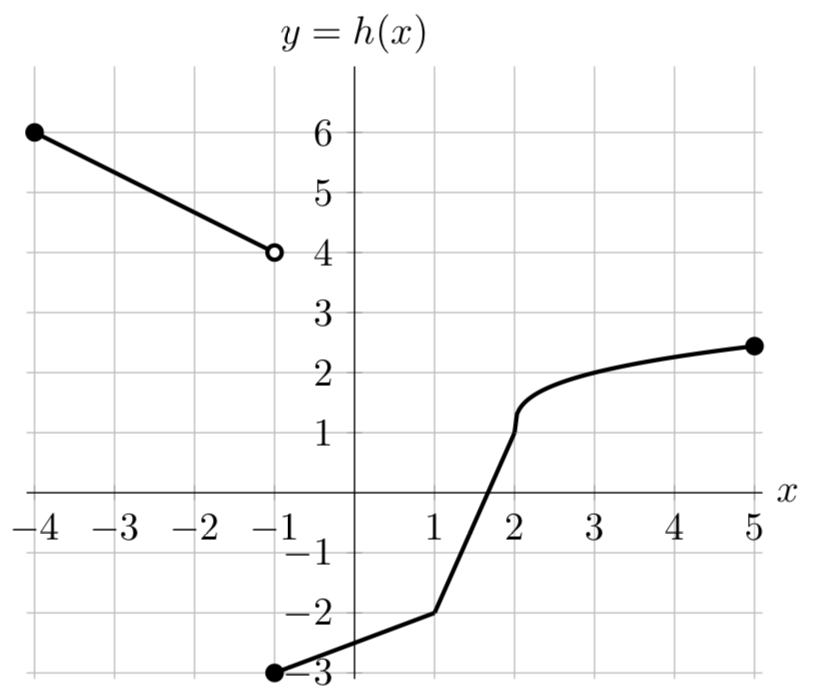
\includegraphics[scale=0.5]{Figures/graphh.png}
          \end{center}
        \end{minipage}
        \begin{minipage}{0.5\linewidth}
          Find the exact value of the following expressions. If there
          is not enough information provided to find the value, write
          NI. If the value does not exist, write DNE. Show all your
          work.
            \begin{enumerate}[(a)]
            \item Let $g(x) = xh(x)$. Find $g'(-2)$.
            \item Let $p(x) = h^{-1}(x)$. Find $p'(0)$.
            \item Find $h'(-1)$.
            \end{enumerate}
        \end{minipage}
        \begin{solution}
          For (a) and (b),\\ see \href{https://dhsp.math.lsa.umich.edu/exams/115exam2/f17/s4.pdf}{https://dhsp.math.lsa.umich.edu/exams/115exam2/f17/s4.pdf}

          For (c), the answer is DNE.
        \end{solution}
\end{questions}
\end{document}
%%% Local Variables:
%%% mode: latex
%%% TeX-master: t
%%% End:
